\section{Auswertung}
\label{sec:Auswertung}

Für die Auswertung der Messergebnisse wird im Folgenden der Mittelwert immer als
\begin{equation*}
  \bar{x} = \frac{1}{N}\sum_{i=1}^{N} x_{i}
\end{equation*}
berechnet und die Standardabweichung mit
\begin{equation*}
  \Delta\bar{x} = \frac{\sigma}{\sqrt{N}} = \sqrt{\frac{1}{N(N-1)}\sum_{i=1}^{N} (x_{i} - \bar{x})^2}.
\end{equation*}
Weiterhin wird die Gaußsche Fehlerfortpflanzung
\begin{equation*}
  \Delta f = \sqrt{\left(\frac{\partial f}{\partial x}\Delta x\right)^2 + \left(\frac{\partial f}{\partial y}\Delta y\right)^2 + \dots}
\end{equation*}
verwendet.

\subsection{Untersuchung des Sättigungsstroms}
Aus den Messwerten lässt sich graphisch ein Sättigungsstrom $I_\text{S}$ ermitteln, der einen
Grenzwert darstellt und auch bei erhöhter Beschleunigungsspannung nicht nennenswert wächst.
Dieser wird zusammen mit den Kennlinien unterschiedlicher Heizströme, welche den Tabellen
(\ref{tab:a20tab}), (\ref{tab:a21tab}), (\ref{tab:a22tab}), (\ref{tab:a23tab}) und (\ref{tab:a24tab}) zu entnehmen sind, 
in Abbildung \ref{fig:plota} dargestellt.
Aus dieser ergeben sich die Sättigungsströme zu
\begin{align*}
  I_\text{2.0} &\approx \SI{0.010}{\milli\ampere}, \\
  I_\text{2.1} &\approx \SI{0.020}{\milli\ampere}, \\
  I_\text{2.2} &\approx \SI{0.042}{\milli\ampere}, \\
  I_\text{2.3} &\approx \SI{0.095}{\milli\ampere}, \\
  I_\text{2.4} &\approx \SI{0.190}{\milli\ampere}.
\end{align*}

\begin{figure}[H]
  \centering
  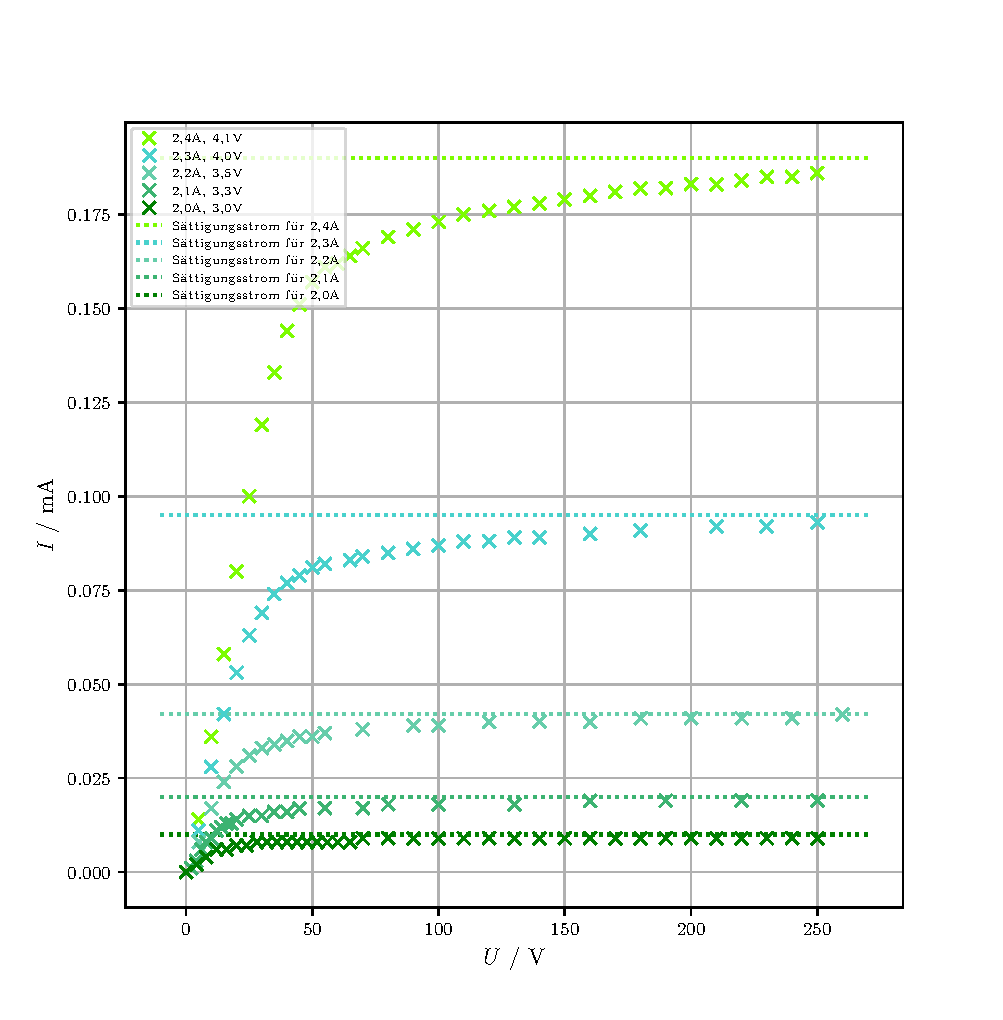
\includegraphics{plota.pdf}
  \caption{Kennlinienschar der Hochvakuumdiode zu variablen Heizströmen. Der Anodenstrom ist in Abhängigkeit von der Beschleunigungsspannung aufgetragen.}
  \label{fig:plota}
\end{figure}

\begin{table}
  \centering
  \caption{Messwerte zur Kennlinie der Hochvakuumdiode bei $\SI{2.0}{\ampere}$ Heizstrom.}
  \label{tab:a20tab}
  \begin{tabular}{S[table-format=3.0] S[table-format=1.3]}
    \toprule
    {$U \:/\: \si{\volt}$} & {$I \:/\: \si{\milli\ampere}$}\\
    \midrule
    0	   & 0.000 \\
    4	   & 0.002 \\
    8	   & 0.004 \\
    12	 & 0.006 \\
    16	 & 0.006 \\
    20	 & 0.007 \\
    24	 & 0.007 \\
    28	 & 0.008 \\
    32	 & 0.008 \\
    36	 & 0.008 \\
    40	 & 0.008 \\
    44	 & 0.008 \\
    48	 & 0.008 \\
    52	 & 0.008 \\
    56	 & 0.008 \\
    60	 & 0.008 \\
    65	 & 0.008 \\
    70	 & 0.009 \\
    80	 & 0.009 \\
    90	 & 0.009 \\
    100	 & 0.009 \\
    110	 & 0.009 \\
    120	 & 0.009 \\
    130	 & 0.009 \\
    140	 & 0.009 \\
    150	 & 0.009 \\
    160	 & 0.009 \\
    170	 & 0.009 \\
    180	 & 0.009 \\
    190	 & 0.009 \\
    200	 & 0.009 \\
    210	 & 0.009 \\
    220	 & 0.009 \\
    230	 & 0.009 \\
    240	 & 0.009 \\
    250	 & 0.009 \\
  \end{tabular}
\end{table}

\begin{table}
  \centering
  \caption{Messwerte zur Kennlinie der Hochvakuumdiode bei $\SI{2.1}{\ampere}$ Heizstrom.}
  \label{tab:a21tab}
  \begin{tabular}{S[table-format=3.0] S[table-format=1.3]}
    \toprule
    {$U \:/\: \si{\volt}$} & {$I \:/\: \si{\milli\ampere}$}\\
    \midrule
    0	  &0.000 \\
    2	  &0.001 \\
    4	  &0.003 \\
    6	  &0.006 \\
    8	  &0.008 \\
    10  &	0.009 \\
    12  &	0.011 \\
    14  &	0.012 \\
    16  &	0.013 \\
    18  &	0.013 \\
    20  &	0.014 \\
    25  &	0.015 \\
    30  &	0.015 \\
    35  &	0.016 \\
    40  &	0.016 \\
    45  &	0.017 \\
    55  &	0.017 \\
    70  &	0.017 \\
    80  &	0.018 \\
    100 & 0.018 \\
    130 & 0.018 \\
    160 & 0.019 \\
    190 & 0.019 \\
    220 & 0.019 \\
    250 & 0.019  \\
  \end{tabular}
\end{table}

\begin{table}
  \centering
  \caption{Messwerte zur Kennlinie der Hochvakuumdiode bei $\SI{2.2}{\ampere}$ Heizstrom.}
  \label{tab:a22tab}
  \begin{tabular}{S[table-format=3.0] S[table-format=1.3]}
    \toprule
    {$U \:/\: \si{\volt}$} & {$I \:/\: \si{\milli\ampere}$}\\
    \midrule
    0	  & 0.000 \\
    5	  & 0.008 \\
    10	& 0.017 \\
    15	& 0.024 \\
    20	& 0.028 \\
    25	& 0.031 \\
    30	& 0.033 \\
    35	& 0.034 \\
    40	& 0.035 \\
    45	& 0.036 \\
    50	& 0.036 \\
    55	& 0.037 \\
    70	& 0.038 \\
    90	& 0.039 \\
    100	& 0.039 \\
    120	& 0.040 \\
    140	& 0.040 \\
    160	& 0.040 \\
    180	& 0.041 \\
    200	& 0.041 \\
    220	& 0.041 \\
    240	& 0.041 \\
    260	& 0.042 \\
   \end{tabular}
\end{table}

\begin{table}
  \centering
  \caption{Messwerte zur Kennlinie der Hochvakuumdiode bei $\SI{2.3}{\ampere}$ Heizstrom.}
  \label{tab:a23tab}
  \begin{tabular}{S[table-format=3.0] S[table-format=1.3]}
    \toprule
    {$U \:/\: \si{\volt}$} & {$I \:/\: \si{\milli\ampere}$}\\
    \midrule
    0	& 0 \\
    5 &	0.011 \\
    10 &	0.028 \\
    15 &	0.042 \\
    20 &	0.053 \\
    25 &	0.063 \\
    30 &	0.069 \\
    35 &	0.074 \\
    40 &	0.077 \\
    45 &	0.079 \\
    50 &	0.081 \\
    55 &	0.082 \\
    65 &	0.083 \\
    70 &	0.084 \\
    80 &	0.085 \\
    90 &	0.086 \\
    100 &	0.087 \\
    110 &	0.088 \\
    120 &	0.088 \\
    130 &	0.089 \\
    140 &	0.089 \\
    160 &	0.090 \\
    180 &	0.091 \\
    210 &	0.092 \\
    230 &	0.092 \\
    250 &	0.093 \\
   \end{tabular}
\end{table}

\begin{table}
  \centering
  \caption{Messwerte zur Kennlinie der Hochvakuumdiode bei $\SI{2.4}{\ampere}$ Heizstrom.}
  \label{tab:a24tab}
  \begin{tabular}{S[table-format=3.0] S[table-format=1.3]}
    \toprule
    {$U \:/\: \si{\volt}$} & {$I \:/\: \si{\milli\ampere}$}\\
    \midrule
    5 &   0.014\\
    10 &  0.036\\
    15 &  0.058\\
    20 &  0.080\\
    25 &  0.100\\
    30 &  0.119\\
    35 &  0.133\\
    40 &  0.144\\
    45 &  0.151\\
    50 &  0.157\\
    55 &  0.161\\
    60 &  0.162\\
    65 &  0.164\\
    70 &  0.166\\
    80 &  0.169\\
    90 &  0.171\\
    100 & 0.173\\
    110 & 0.175\\
    120 & 0.176\\
    130 & 0.177\\
    140 & 0.178\\
    150 & 0.179\\
    160 & 0.180\\
    170 & 0.181\\
    180 & 0.182\\
    190 & 0.182\\
    200 & 0.183\\
    210 & 0.183\\
    220 & 0.184\\
    230 & 0.185\\
    240 & 0.185\\
    250 & 0.186\\
   \end{tabular}
\end{table}

\subsection{Untersuchung des Langmuir-Schottkyschen Raumladungsgesetzes}
Zur Untersuchung des Raumladungsgebietes werden die Messpaare des höchsten Heizstroms
$I = 2,4\,\si{\ampere}$ aus Tabelle (\ref{tab:a24tab}) in Abbildung (\ref{fig:plotb}) 
doppeltlogarithmisch gegeneinander aufgetragen.
Es findet eine lineare Ausgleichsrechnung der Form 
\begin{align*}
\ln(I) = a\cdot \ln(U) + \ln(b)
\end{align*}
statt, bei der $a$ den Exponenten der Strom-Spannungsbeziehung darstellt. Mittels dieser
ergibt sich
\begin{align*}
a &= (1,12 \pm 0,03), \\
b &= (0,0028 \pm 0,0002).
\end{align*}

\begin{figure}[H]
  \centering
  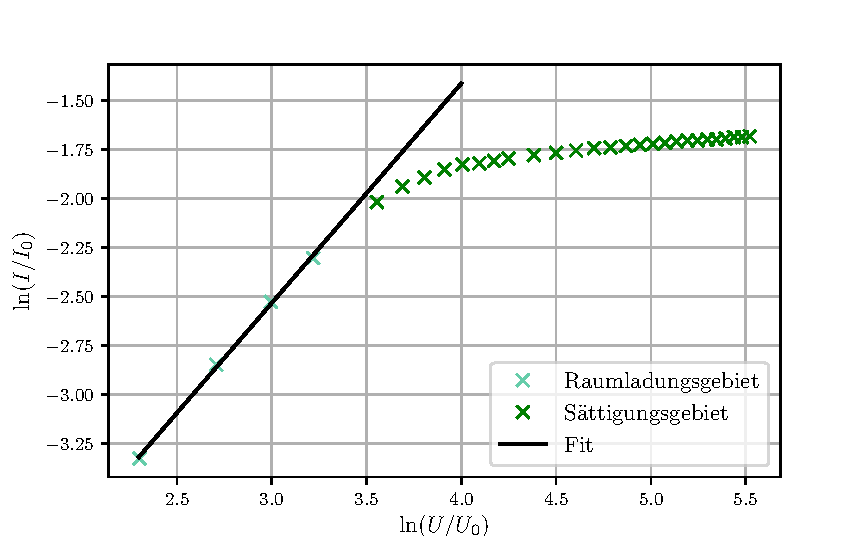
\includegraphics{plotb.pdf}
  \caption{Doppeltlogarithmische Kennlinie der Hochvakuumdiode bei einem Heizstrom von $\SI{2.4}{\ampere}$.}
  \label{fig:plotb}
\end{figure}

\subsection{Untersuchung des Anlaufstromgebiets}
Um das Anlaufstromgebiet zu untersuchen, müssen die gemessenen Spannung entsprechend
dem Spannungsabfall an dem Innenwiderstand des Nanoamperemeters $R_\text{Innen} = 1\,\si{\mega\ohm}$
über
\begin{align*}
U_\text{Korrektur} = U + U_\text{R} = U + R_\text{Innen} I
\end{align*}
korrigiert werden. Die korrigierten Messwerte sind in Tabelle (\ref{tab:tabc}) aufgelistet und werden
zusammen mit einer Ausgleichsgeraden der Form
\begin{align*}
\ln(I) = A\cdot U + \ln(B)
\end{align*} 
in Abbildung (\ref{fig:plotc}) dargestellt. Aus der Ausgleichsrechnung ergibt sich
\begin{align*}
A &= (-5,08 \pm 0,05)\,\si{\per\volt},\\
B &= (50,32 \pm 1,46).
\end{align*}

Aus Gleichung xyz wird deutlich, dass
\begin{align*}
  A &= -\frac{\symup{e_\text{0}}}{\symup{k_\text{B}} T}, \\
  B &= j_0 \cdot \exp\left(-\frac{\symup{e_\text{0}} \phi_\text{A}}{\symup{k_\text{B}} T}\right) = \mathit{const}.
\end{align*}

Daraus ergibt sich eine Kathodentemperatur von
\begin{align*}
T = (2286 \pm 21)\,\si{\kelvin}.
\end{align*}

\begin{figure}[H]
  \centering
  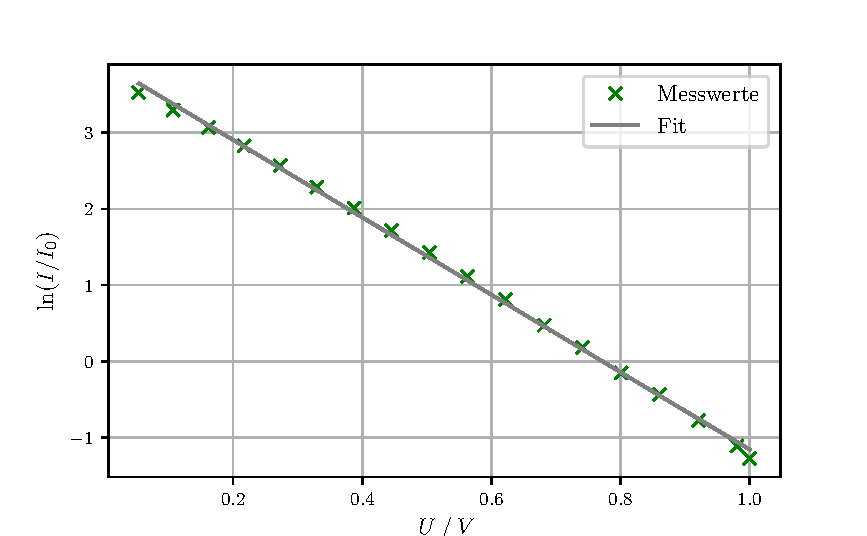
\includegraphics{plotc.pdf}
  \caption{Einfach logarithmische Darstellung der Messwerte zum Anlaufstromgebiet.}
  \label{fig:plotc}
\end{figure}

\begin{table}
  \centering
  \caption{Messwerte zur Untersuchung des Anlaufstromgebiets einer Hochvakuumdiode mit Heizstrom $I = \SI{2.4}{\volt}$.}
  \label{tab:tabc}
  \begin{tabular}{S[table-format=1.2] S[table-format=1.3] S[table-format=2.2]}
    \toprule
    {$U_\text{Messung} \:/\: \si{\volt}$} & {$U \:/\: \si{\volt}$} & {$I \:/\: \si{\nano\ampere}$}\\
    \midrule
    0.02 & 0.054  &  34.0 \\
    0.08 & 0.107  &  27.0 \\
    0.14 & 0.162  &  21.5 \\
    0.20 & 0.217  &  16.9 \\
    0.26 & 0.273  &  13.0 \\
    0.32 & 0.333  &  9.80 \\
    0.38 & 0.387  &  7.47 \\
    0.44 & 0.446  &  5.55 \\
    0.50 & 0.504  &  4.15 \\
    0.56 & 0.563  &  3.05 \\
    0.62 & 0.622  &  2.25 \\
    0.68 & 0.682  &  1.60 \\
    0.74 & 0.741  &  1.20 \\
    0.80 & 0.801  &  0.86 \\
    0.86 & 0.861  &  0.65 \\
    0.92 & 0.920  &  0.46 \\
    0.98 & 0.980  &  0.33 \\
    1.00 & 1.000  &  0.28 \\
  \end{tabular}
\end{table}

\subsection{Bestimmung der Kathodentemperatur aus der Leistungsbilanz}
Aus der Leistungsbilanz des Heizstromkreises lässt sich die Temperatur der Glühkathode ebenfalls bestimmen.
Die zugeführte Leistung
\begin{equation*}
  N_\text{zu} = V_f \cdot I_f
\end{equation*}
entspricht der Summe der über die Apparatur abgegebenen Wärmeleistung $N_\text{W} = \SI{0.9}{\watt}$ und der Strahlungsleistung
\begin{equation*}
  N_\text{W} = f \eta \symup{\sigma} T^4,
\end{equation*}
welche über das Stefan-Boltzmann-Gesetz bestimmt wird, wobei
\begin{align*}
  \symup{\sigma} &= \SI{5.7e-12}{\watt\per\centi\meter\squared\kelvin\squared}, \\
  f &= \SI{0.35}{\centi\meter\squared}, \\
  \eta &=\num{0.28},
\end{align*}
mit der Stefan-Boltzmann-Konstante $\symup{\sigma}$, der Kathodenoberfläche $f$ und dem Emissionsvermögen $\eta$.
Für die Temperatur ergibt sich aus der Leistungsgleichung also

\begin{equation*}
T=\sqrt[4]{\frac{I_f V_f-0.9}{f \eta \symup{\sigma}}}.
\end{equation*}

Die berechneten Temperaturen sind in Tabelle \ref{tab:tabT} aufgeführt.
\begin{table}
  \centering
  \caption{Glühkathodentemperaturen zu Kennlinienmessungen einer Wolframkatode.}
  \label{tab:tabT}
  \begin{tabular}{S[table-format=1.1] S[table-format=1.1] S[table-format=4.2]}
    \toprule
    {$U_\text{Heiz} \:/\: \si{\volt}$} & {$I_\text{Heiz} \:/\: \si{\ampere}$} & {$T \:/\: \si{\kelvin}$}\\
    \midrule
    3.0  &   2.0   &   1738.27 \\
    3.3  &   2.1   &   1812.61 \\
    3.5  &   2.2   &   1867.89 \\
    4.0  &   2.3   &   1963.33 \\
    4.1  &   2.4   &   2000.13 \\
%T =  [1738.27030514 1812.60884626 1867.89300329 1963.33446436 2000.13425071]
\end{tabular}
\end{table}

Gemittelt ergibt sich für die Kathodentemperatur somit
\begin{equation*}
  T = \SI{1876 \pm 48}{\kelvin}.
\end{equation*}

\subsection{Bestimmung der Austrittsarbeit von Wolfram}
Aus den soeben bestimmten Temperaturen der Kathode sowie der Sättigungsströme lässt sich durch Umstellen der
Gleichung (5) die Austrittsarbeit von Wolfram bestimmen:
\begin{equation*}
  \symup{e}_0 \phi = -\ln\left(\frac{I_s \symup{h}^3}{4 \pi \symup{e}_0 \symup{m}_0 \symup{k}_B^2 f T^2}\right)\symup{k}_B T,
\end{equation*}
mit der Elementarladung $\symup{e}_0$ und der Ruhemasse $\symup{m}_0$ des Elektrons
\begin{align*}
  \symup{e}_0 &= \SI{1.602e-19}{\coulomb}, \\
  \symup{m}_0 &= \SI{9.109e-31}{\kilo\gram},
\end{align*}
welche in Tabelle (\ref{tab:tabW}) aufgelistet sind.
\begin{table}[H]
  \centering
  \caption{Temperaturabhängige Austrittsarbeit einer Wolframkathode.}
  \label{tab:tabW}
  \begin{tabular}{S[table-format=4.2] S[table-format=1.1] S[table-format=1.2]}
    \toprule
    {$T \:/\: \si{\kelvin}$} & {$I_\text{S} \:/\: \si{\milli\ampere}$} & {$W \:/\: \si{\eV}$}\\
    \midrule
    1738.27  &   0.010  &   4.52 \\
    1812.61  &   0.020  &   4.62 \\
    1867.89  &   0.042  &   4.64 \\
    1963.33  &   0.095  &   4.76 \\
    2000.13  &   0.190  &   4.72 \\
%W =  [4.51973815 4.61784201 4.63782766 4.75656624 4.72424343]
  \end{tabular}
\end{table}
Gemittelt ergibt sich eine Austrittsarbeit für Wolfram von
\begin{align*}
W = (4,65 \pm 0,08)\,\si{\eV}.
\end{align*}